% Preamble
\documentclass[11pt]{article}

% Packages
\usepackage{graphicx} % Required for inserting images
\usepackage{xcolor,colortbl}
\usepackage[a4paper, margin=1in]{geometry}
\usepackage[utf8]{inputenc}
\usepackage{blindtext}
\usepackage[english]{babel}
%%%%%%%%%%%%%%%%%%%%%%%%%%%%%%%%%%%%%%%%%%%%%%%%%%%%%%%%%%%%%%%%%%%%%%%%%
% This section is based on the bbk10.clo file
% of Palash Baran Pal's bangtex
% http://www.saha.ac.in/theory/palashbaran.pal/bangtex/bangtex.html
%%%%%%%%%%%%%%%%%%%%%%%%%%%%%%%%%%%%%%%%%%%%%%%%%%%%%%%%%%%%%%%%%%%%%%%%%

\def\sbng{\bngviii}
\def\tbng{\bngvi}
\def\bng{\bngx}
\def\lbng{\bngxiv}
\def\Lbng{\bngxviii}
\def\LBng{\bngxxii}
\def\hbng{\bngxxv}
\def\Hbng{\bngxxx}
%
\def\sbns{\bnsviii}
\def\tbns{\bnsvi}
\def\bns{\bnsx}
\def\lbns{\bnsxiv}
\def\Lbns{\bnsxviii}
\def\LBns{\bnsxxii}
\def\hbns{\bnsxxv}
\def\Hbns{\bnsxxx}
%
\def\sbnw{\bnwviii}
\def\tbnw{\bnwvi}
\def\bnw{\bnwx}
\def\lbnw{\bnwxiv}
\def\Lbnw{\bnwxviii}
\def\LBnw{\bnwxxii}
\def\hbnw{\bnwxxv}
\def\Hbnw{\bnwxxx}


%%%%%%%%%%%%%%%%%%%%%%%%%%%%%%%%%%%%%%%%%%%%%%%%%%%%%%%%%%%%%%%%%%%%%%%%%
% This section is based on the bangfont.tex file
% of Palash Baran Pal's bangtex
% http://www.saha.ac.in/theory/palashbaran.pal/bangtex/bangtex.html
%%%%%%%%%%%%%%%%%%%%%%%%%%%%%%%%%%%%%%%%%%%%%%%%%%%%%%%%%%%%%%%%%%%%%%%%%

%%
%% Defining the normal bangla fornts
%%

\font\bngv=bang10 scaled 500
\font\bngvi=bang10 scaled 600
\font\bngvii=bang10 scaled 700
\font\bngviii=bang10 scaled 800
\font\bngix=bang10 scaled 900
\font\bngx=bang10
\font\bngxi=bang10 scaled 1100
\font\bngxii=bang10 scaled 1200
\font\bngxiv=bang10 scaled 1400
\font\bngxviii=bang10 scaled 1800
\font\bngxxii=bang10 scaled 2200
\font\bngxxv=bang10 scaled 2500
\font\bngxxx=bang10 scaled 3000

%%
%% Defining the slanted bangla fonts
%%
\font\bnsv=bangsl10 scaled 500
\font\bnsvi=bangsl10 scaled 600
\font\bnsvii=bangsl10 scaled 700
\font\bnsviii=bangsl10 scaled 800
\font\bnsix=bangsl10 scaled 900
\font\bnsx=bangsl10
\font\bnsxi=bangsl10 scaled 1100
\font\bnsxii=bangsl10 scaled 1200
\font\bnsxiv=bangsl10 scaled 1400
\font\bnsxviii=bangsl10 scaled 1800
\font\bnsxxii=bangsl10 scaled 2200
\font\bnsxxv=bangsl10 scaled 2500
\font\bnsxxx=bangsl10 scaled 3000

%%
%% Defining the wide bangla fonts
%%
\font\bnwv=bangwd10 scaled 500
\font\bnwvi=bangwd10 scaled 600
\font\bnwvii=bangwd10 scaled 700
\font\bnwviii=bangwd10 scaled 800
\font\bnwix=bangwd10 scaled 900
\font\bnwx=bangwd10
\font\bnwxi=bangwd10 scaled 1100
\font\bnwxii=bangwd10 scaled 1200
\font\bnwxiv=bangwd10 scaled 1400
\font\bnwxviii=bangwd10 scaled 1800
\font\bnwxxii=bangwd10 scaled 2200
\font\bnwxxv=bangwd10 scaled 2500
\font\bnwxxx=bangwd10 scaled 3000


%%
%% Inhibiting linebreak within words
%%
%\hyphenpenalty=10000 \pretolerance=-1 \tolerance=10000

%%
%% Defining the macro for e-kar, i-kar etc
%%
\def\*#1*#2{o\null{#2}{#1}}

%%
%% Redefining some macros to make them consistent with bangla fonts
%%
\def\d#1{\oalign{\smash{#1}\crcr\hidewidth{$\!$\rm.}\hidewidth}}


%%
%% Emulating the bold font
%%
\def\sh#1{\setbox0=\hbox{#1}%
     \kern-.02em\copy0\kern-\wd0
     \kern.04em\copy0\kern-\wd0
     \kern-.02em\raise.0433em\box0 }
\usepackage{multirow}
\usepackage{multicol}
\usepackage{enumitem}
\usepackage{float}
\usepackage{mathtools}
\usepackage{amsmath}
\usepackage[numbers]{natbib}
\usepackage{tikz}
\usetikzlibrary{arrows.meta}
\usetikzlibrary{shapes.geometric, calc}
\usepackage{pgfplots}
\usepackage{pgfplotstable}
\pgfplotsset{compat=1.7}
\usepackage{algorithm}
\usepackage{algpseudocode}
\usepackage{amsfonts}



\title{Extractive Text Summarization Using Word Similarity Based Spectral Clustering}
\author{Fahim Morshed, Md. Abdur Rahman, Sumon Ahmed}


% Document
\begin{document}

    \maketitle
    \setlength{\parindent}{0pt}
    \begin{abstract}
        Extractive Text Summarization is the process of picking the best parts of
        a larger text without losing any key information.
        This is really necessary in this day and age to get concise information
        faster due to digital information overflow.
        But research in this field, specially in Bengali, has been inadequate.
        This papers objective is to develop an extractive text summarization
        method for Bengali language, that uses the latest NLP techniques
        and can be extended to other low resource languages.
        We developed a word Similarity-based Spectral Clustering (WSbSC) method
        for Bengali extractive text summarization.
        It extracts key sentences by grouping semantically similar sentences into clusters
        with a novel sentence similarity calculating algorithm.
        We took the geometric means of individual Gaussian similarity of Word embedding vectors.
        Then used TF-IDF ranking to pick the best sentence from each cluster.
        We tested this method on four different Bengali text summarization datasets,
        and it outperformed other recent models on every ROUGE metric on average by 43.2\%.
        We also experimented the method on Turkish, Marathi and Hindi language and found that the
        performance on those languages often exceeded the performance of Bengali.
        We also provide a new high quality dataset for text summarization evaluation.
        We believe this research is a crucial addition to Bengali Natural Language Processing,
        that can easily be extended into other languages.
    \end{abstract}

    \section{Introduction}\label{sec:introduction}
    Automatic Text Summarization (ATS) is a major area of natural language processing (NLP) that aims
to automatically shorten a document or a set of documents into a shorter version, while keeping all
the key information~\cite{Widyassari-2022-rev-ats-tech-met}.
This task has become more and more important in the current digital age, where the amount of textual
data grows exponentially in many fields, such as news, legal documents, health reports, research papers,
and social media content.
ATS techniques allow users to quickly get the essential information without needing to read through large
amounts of text~\cite{wafaa-2021-summary-comprehensive-review}.\\

There are two main types of text summarization: extractive and abstractive~\cite{tas-2017-rev-text-sum-2}.
Extractive summarization, which is the focus of this paper, works by selecting best sentences or phrases directly
from the source document, maintaining the original wording and sentence structure~\cite{moratanch-2017-extractive-review}.
This is in contrast to abstractive summarization, which involves generating new sentences to capture the meaning of the
text, similar we may summarize~\cite{Moratanch-2016-abstractive-rev}.
Extractive summarization is widely used because of its simplicity and effectiveness, especially for languages with
limited NLP resources~\cite{gupta-2010-extractive-rev}.\\

Text summarization is used in many fields, from automatic news summarization, content filtering, and recommendation
systems to assisting legal professionals in going through long documents and researchers in reviewing academic papers.
It can also play a critical role in personal assistants and chatbots, providing condensed information to users quickly
and efficiently~\cite{tas-2017-rev-text-sum-2}.\\

A commonly used method for extractive text summarization is graph-based summarization.
This method represents the sentences of a document as nodes of a graph, and the edges between them are weighted by the
similarity between the sentences~\cite{wafaa-2021-summary-comprehensive-review}.
Popular algorithms like LexRank~\cite{Erkan-lexRank-2004} and TextRank~\cite{mihalcea-2004-textrank} build graphs based
on cosine similarity between sentence embeddings and apply ranking algorithms such as PageRank~\cite{page-PageRank-1999} in
case of LexRank~\cite{Erkan-lexRank-2004} or Random Walk in case of TextRank~\cite{mihalcea-2004-textrank} to
determine which sentences are the most important.
These sentences are then selected to make the summary.
Graph-based methods offer a more robust way to capture sentence importance and relationship, ensuring that the
extracted summary covers the key information while minimizing redundancy~\cite{wafaa-2021-summary-comprehensive-review}.\\

A subset of graph-based approach to extractive summarization is clustering-based summarization.
Here, sentences are grouped into clusters based on their semantic similarity, and one representative sentence from each
cluster is chosen to form the summary~\cite{Mohan-2022-topic-modeling-rev-clustering}.
Clustering reduces redundancy by ensuring that similar sentences are grouped together and that only the most
representative sentence is selected.
This method is effective in documents that cover multiple topics or subtopics, as it allows the summary to touch on
each area without being repetitive.\\

For Bengali, a low-resource language, early attempts at text summarization relied on traditional methods like TF-IDF
(Term Frequency-Inverse Document Frequency) scoring~\cite{das-2022-tfidf,sarkar-2012-tfidf}.
These approaches, while simple, faced challenges in capturing the true meaning of sentences, as they treated words as
isolated terms~\cite{tas-2017-rev-text-sum-2}.
Graph-based methods introduced improvements by incorporating sentence similarity, but they were still limited by the
quality of the embeddings used for the Bengali language.
With the advent of word embedding models like FastText~\cite{grave-etal-2018-fasttext}, which supports over 157
languages, including Bengali, it became possible to represent words in a Vector Space Model, thus enabling
more accurate sentence similarity calculations.\\

However, existing models that use word embeddings, such as \citeauthor{roychowdhury-etal-2022-spectral-base}’s
\cite{roychowdhury-etal-2022-spectral-base} Sentence Average Similarity-based Spectral Clustering (SASbSC) method,
encountered issues when averaging word vectors to represent sentence meaning.
This method failed in most cases because words in a sentence are often complementary rather than being similar, leading
to inaccurate sentence representations when averaging their vectors.
As a result, important word-to-word relationships between sentences were lost, reducing the effectiveness of the method.\\

In this paper, we propose a new approach to address these challenges.
Our method improves upon previous attempts by focusing on the individual similarity between words in sentences rather
than averaging word vectors.
Here the gaussian similarities between each word and the Most Similar Word from the other sentence for that word are
used to get the similarity between the two sentence.
This method captures the true semantic relationships between sentences more effectively.
By applying Gaussian similarity to the Most Similar Word Distance ($D_{msw}$) values, we build an affinity matrix that
better reflects sentence closeness.
We then apply spectral clustering on this matrix to group similar sentences together and use TF-IDF to select the
most representative sentences from each cluster.
This approach reduces redundancy and improves the quality of the summary by selecting sentences that are not only
relevant but also diverse.
This method works really well for Bengali on four different diverse datasets consistently.
It consistently outperforms other graph based methods like BenSumm~\cite{chowdhury-etal-2021-tfidf-clustering},
SASbSC~\cite{roychowdhury-etal-2022-spectral-base}, LexRank~\cite{Erkan-lexRank-2004}.
It also performs similarly well on every other low resource languages we tried it on.
These languages are Hindi, Marathi and Turkish.
These are the languages where reliable evaluation datasets could be found to test the effectiveness.\\

In summary, this paper contributes a novel methodology for extractive text summarization for the Bengali language by
improving sentence similarity calculations and enhancing clustering techniques.
It addresses the limitations of previous models, such as misleading word vector averages~\cite{roychowdhury-etal-2022-spectral-base},
and offers a better solution for creating less redundant and information rich summaries.
Through this work, we aim to improve the performance of Bengali text summarization systems and contribute to the
growing field of NLP for low-resource languages.

    \section{Literature Review}\label{sec:literature-review}
    Text Summarization has been an important necessity for textual data consumption for a long time.
But manually summarizing is really time-consuming and counter-productive.
So automating the Text Summarization process has been a research problem for a long time.
Attempts at automatic text summarization started with indexing-based methods~\cite{Baxendale_1958_firstsummarization}.
In this attempt \citeauthor{Baxendale_1958_firstsummarization}~\cite{Baxendale_1958_firstsummarization} attempted to
summarize text by scoring sentences higher based on a certain word list.
But this type of method failed to capture the topic and essence of the input text.
To solve this, Text Summarization with statistical methods like TF-IDF became very popular.
\citeauthor{edmundson_1969_earlysum}~\cite{edmundson_1969_earlysum} proposed a method which can focus on the central topic of a document.
It uses two metrics, Term Frequency (how many times a term appears in the input) and Inverse Document Frequency
(inverse of how many documents the term appears in a corpus) to calculate the importance of a term in a document.
This method identifies the words that are common in the input text but not as common in the language and identifying
them as the central topic.
But it was too error-prone due to it thinking every word as a unique isolated term and not having
any semantic relation with other words.
Some words may be a central topic of a document but not identified as such because they got divided into too many
synonyms. \\

Modern breakthroughs into the extractive text summarization began with the usage of Graph-based Extractive
Text Summarization methods like LexRank~\cite{Erkan-lexRank-2004} or TextRank~\cite{mihalcea-2004-textrank}.
LexRank~\cite{Erkan-lexRank-2004} calculates the similarity between two sentences using cosine similarity
and builds a graph
containing similarity between every pair of sentences in the input.
The most important sentences are then identified using the PageRank~\cite{page-PageRank-1999} algorithm on the graph.
This algorithm ranked the sentences, who are most similar with other high ranked sentences, higher.
TextRank~\cite{mihalcea-2004-textrank} also uses a similar approach,
but for every sentence, the method distributed its scores to its neighbours using a random walk.
The process was done over and over until the scores converge.
Although these models are very novel compared to their time, they still lacked fundamental understanding of the
words involved in a sentence.\\

To solve this problem by better expressing the similarity between words,
a mathematical abstraction called Word Vector Embedding was conceptualized by the seminal
work of \citeauthor{salton-1975-word-vector}~\cite{salton-1975-word-vector}.
Word Vector Space is a mathematical abstraction of a vocabulary where the closer two words
are meaning-wise, the closer they are in the vector space.
Using word vector for summarization has only been started
to be attempted recently~\cite{Jain-2017-word-vector-embedding-summary}.\\

But Text Summarization attempts in Bengali are a more recent development than in other high resource languages.
So, a lot of sophisticated approaches from other languages haven't been attempted yet.
Earlier Extractive methods have been focused on some derivative of TF-IDF based text
summarization such as \citeauthor{chowdhury-etal-2021-tfidf-clustering}~\cite{chowdhury-etal-2021-tfidf-clustering},
\citeauthor{das-2022-tfidf}~\cite{das-2022-tfidf}, \citeauthor{sarkar-2012-tfidf}~\cite{sarkar-2012-tfidf}.
\citeauthor{sarkar-2012-tfidf}~\cite{sarkar-2012-tfidf} used simple TF-IDF score of each sentence to rank them and
pick the best sentences.
\citeauthor{das-2022-tfidf}~\cite{das-2022-tfidf} used weighted TF-IDF along with some other features like sentence position
to rank the sentences.
\citeauthor{chowdhury-etal-2021-tfidf-clustering}~\cite{chowdhury-etal-2021-tfidf-clustering} however, used TF-IDF
matrix of a document to build a graph and perform Hierarchical Clustering to group sentences together and pick one
sentence from each group.
One shortcoming of this model is that TF-IDF matrix is not semantically equivalent to the actual sentences.
So it didn't perfectly represent the sentences' semantic closeness in the graph.
Using Word Vector Embedding for Bengali has solved this problem.
FastText~\cite{grave-etal-2018-fasttext} released a dataset\footnote{\textit{https://fasttext.cc/docs/en/crawl-vectors.html}}
that had word vector embedding in 157 languages, including Bengali.
Using this dataset, \citeauthor{roychowdhury-etal-2022-spectral-base}~\cite{roychowdhury-etal-2022-spectral-base}
proposed a model where they replaced all the words with their respective vector, then averaged the vectors in a
sentence to get the vector for a sentence.
The Gaussian Similarity between the vectors is used to build the graph.
On the graph, spectral clustering was used to group them together and pick one sentence from each cluster using cosine
similarity to get the summary.\\

\begin{figure}
    \centering
    \begin{tikzpicture}[scale=0.001\textwidth]
    \newcommand{\xleft}{2};
    \newcommand{\ytop}{11};
    \newcommand{\xright}{14};
    \newcommand{\ybot}{0};
    % Draw quarters
    \draw (\xleft,\ytop) rectangle (\xleft+10,\ytop+10);
    \draw (\xright,\ytop) rectangle (\xright+10,\ytop+10);
    \draw (\xleft,\ybot) rectangle (\xleft+10,\ybot+10);
    \draw (\xright,\ybot) rectangle (\xright+10,\ybot+10);

    % Add labels
    \node at (0.95,16.15) {(a)};
    \node at (12.95,16.15) {(b)};
    \node at (0.95,5.15) {(c)};
    \node at (12.95,5.15) {(d)};

    %set a
    \newcommand{\aax}{0.25};\newcommand{\aay}{0.35};
    \newcommand{\abx}{0.25};\newcommand{\aby}{5.8};
    \newcommand{\acx}{5};\newcommand{\acy}{0.5};
    \newcommand{\adx}{4.5};\newcommand{\ady}{9.5};
    \newcommand{\aex}{5.5};\newcommand{\aey}{9.6};
    \newcommand{\afx}{9.5};\newcommand{\afy}{0.5};
    %set b
    \newcommand{\bax}{1.5};\newcommand{\bay}{4};
    \newcommand{\bbx}{4.5};\newcommand{\bby}{8.5};
    \newcommand{\bcx}{6.5};\newcommand{\bcy}{1};
    \newcommand{\bdx}{8.2};\newcommand{\bdy}{7.8};
    %set c
    \newcommand{\cax}{2.8};\newcommand{\cay}{4};
    \newcommand{\cbx}{4.2};\newcommand{\cby}{6.2};
    \newcommand{\ccx}{6.2};\newcommand{\ccy}{5};
    \newcommand{\cdx}{6.5};\newcommand{\cdy}{4};

    %set a at a
    \fill[blue] (\xleft+\aax,\ytop+\aay) circle(.15);
    \fill[blue] (\xleft+\abx,\ytop+\aby) circle(.15);
    \fill[blue] (\xleft+\acx,\ytop+\acy) circle(.15);
    \fill[blue] (\xleft+\adx,\ytop+\ady) circle(.15);
    \fill[blue] (\xleft+\aex,\ytop+\aey) circle(.15);
    \fill[blue] (\xleft+\afx,\ytop+\afy) circle(.15);
    %set a at b
    \fill[blue] (\xright+\aax,\ytop+\aay) circle(.15);
    \fill[blue] (\xright+\abx,\ytop+\aby) circle(.15);
    \fill[blue] (\xright+\acx,\ytop+\acy) circle(.15);
    \fill[blue] (\xright+\adx,\ytop+\ady) circle(.15);
    \fill[blue] (\xright+\aex,\ytop+\aey) circle(.15);
    \fill[blue] (\xright+\afx,\ytop+\afy) circle(.15);
    %set a at c
    \fill[blue] (\xleft+\aax,\ybot+\aay) circle(.15);
    \fill[blue] (\xleft+\abx,\ybot+\aby) circle(.15);
    \fill[blue] (\xleft+\acx,\ybot+\acy) circle(.15);
    \fill[blue] (\xleft+\adx,\ybot+\ady) circle(.15);
    \fill[blue] (\xleft+\aex,\ybot+\aey) circle(.15);
    \fill[blue] (\xleft+\afx,\ybot+\afy) circle(.15);

    \newcommand{\amx}{\aax/6+\abx/6+\acx/6+\adx/6+\aex/6+\afx/6};
    \newcommand{\amy}{\aay/6+\aby/6+\acy/6+\ady/6+\aey/6+\afy/6};
    \draw[blue] (\xleft+\amx,\ybot+\amy) circle (0.15);
    %set a at d
    \fill[blue] (\xright+\aax,\ybot+\aay) circle(.15);
    \fill[blue] (\xright+\abx,\ybot+\aby) circle(.15);
    \fill[blue] (\xright+\acx,\ybot+\acy) circle(.15);
    \fill[blue] (\xright+\adx,\ybot+\ady) circle(.15);
    \fill[blue] (\xright+\aex,\ybot+\aey) circle(.15);
    \fill[blue] (\xright+\afx,\ybot+\afy) circle(.15);

    \draw[blue] (\xright+\amx,\ybot+\amy) circle (0.15);
    %set b at a
    \fill[red] (\xleft+\bax,\ytop+\bay) circle(.15);
    \fill[red] (\xleft+\bbx,\ytop+\bby) circle(.15);
    \fill[red] (\xleft+\bcx,\ytop+\bcy) circle(.15);
    \fill[red] (\xleft+\bdx,\ytop+\bdy) circle(.15);
    %set b at c
    \fill[red] (\xleft+\bax,\ybot+\bay) circle(.15);
    \fill[red] (\xleft+\bbx,\ybot+\bby) circle(.15);
    \fill[red] (\xleft+\bcx,\ybot+\bcy) circle(.15);
    \fill[red] (\xleft+\bdx,\ybot+\bdy) circle(.15);

    \newcommand{\bmx}{\bax/4+\bbx/4+\bcx/4+\bdx/4};
    \newcommand{\bmy}{\bay/4+\bby/4+\bcy/4+\bdy/4};
    \draw[red] (\xleft+\bmx,\ybot+\bmy) circle (0.15);
    %set c at b
    \fill[red] (\xright+\cax,\ytop+\cay) circle(.15);
    \fill[red] (\xright+\cbx,\ytop+\cby) circle(.15);
    \fill[red] (\xright+\ccx,\ytop+\ccy) circle(.15);
    \fill[red] (\xright+\cdx,\ytop+\cdy) circle(.15);
    %set c at d
    \fill[red] (\xright+\cax,\ybot+\cay) circle(.15);
    \fill[red] (\xright+\cbx,\ybot+\cby) circle(.15);
    \fill[red] (\xright+\ccx,\ybot+\ccy) circle(.15);
    \fill[red] (\xright+\cdx,\ybot+\cdy) circle(.15);

    \newcommand{\cmx}{\cax/4+\cbx/4+\ccx/4+\cdx/4};
    \newcommand{\cmy}{\cay/4+\cby/4+\ccy/4+\cdy/4};
    \draw[red] (\xright+\cmx,\ybot+\cmy) circle (0.15);

    %drawing line
    \draw[green] (\xleft+\amx,\ybot+\amy) --  (\xleft+\bmx,\ybot+\bmy);
    \draw[green] (\xright+\amx,\ybot+\amy) --  (\xright+\cmx,\ybot+\cmy);

\end{tikzpicture}
    \caption{Scenarios where averaging method fails.}
    \label{fig:sarkar-problem}
\end{figure}

But this model also had a critical weakness.
Words in a sentence do not have similar meaning, instead they express different parts of one whole meaning of a sentence.
Which means they are complementary instead of being similar.
So word averages always tend to be in the center and don't represent the semantic similarity anymore because the word
vectors get scattered throughout the vector space due to this complementary nature.
An example is shown in Figure~\ref{fig:sarkar-problem} where the distance between the average word vectors is being
misleading.
In the figure, each point represents a word vector.
The words from the same sentence are grouped together by being colored the same.
In Figure~\ref{fig:sarkar-problem}(a), a scenario is shown in which the words of the two sentences are closer
together in a vector space.
The average distance between these two sentences can be seen in the Figure~\ref{fig:sarkar-problem}(c).
We can see that averaging the words made both of the average clusters in the center.
In Figure~\ref{fig:sarkar-problem}(b), we can see a different scenario where the word vectors are farther apart meaning wise.
But the Figure~\ref{fig:sarkar-problem}(d) shows the average vector for these two sentences is closer than in the first
scenario, thus making this metric misleading.
This shortcoming has been one of the key motivations for this research.

    \section{Methodology}\label{sec:methodology}
    The summarization process followed here can be boiled down as, grouping together all the close sentences
together based on their meaning and then picking one sentence from each group to minimize redundancy
and maximize sentence coverage.
Often most widely used extractive summarization methods involve scoring the sentences based on some metric and
then picking the best scoring sentences to generate the summaries~\cite{das-2022-tfidf,sarkar-2012-tfidf}.
But in a single topic text document it often picks similar sentences creating redundancy due to all of them having the
central topic terms.
To mitigate this, firstly grouped the sentences with similar meaning together and then finally picked one
sentence from each group to generate a summary.
This will ensure maximum coverage of topics while also reducing redundancy.
This method has also been tried before by \citeauthor{roychowdhury-etal-2022-spectral-base}~\cite{roychowdhury-etal-2022-spectral-base}.
But the main challenge to reducing the redundancy is to develop a method that can accurately predict how close the
meaning of the two sentences are.
In this paper, we propose a method that can do it.
The summarization process followed here involves total 4 steps.
These are, in order of their use, Pre-processing, Sentence similarity calculation, Clustering and Summary generation.
These steps are further discussed in the following subsections.

\subsection{Pre-processing}\label{subsec:pre-processing}
Pre-processing is a standard step in Natural Language Processing that transforms the raw human language
inputs into a format that can be used by a computer algorithm.
Here the input document is transformed into a list of sets of vectors where each word is represented
with a vector, each sentence as a set of vectors and the whole document as a list of said sets.
The Pre-processing involves 3 steps.
These are Tokenization, Stop Word Removal, Word Embedding.
A very common step in Pre-processing, Word Stemming, isn't used in here as the word embedding dataset
works best for the whole word instead of the stemmed word.
These steps are further discussed bellow.
This whole process is shown in Algorithm~\ref{alg:preprocessing}.

\subsubsection{Tokenization}
Tokenization is the step of dividing an input document into sentences and words in a usable format.
Here the input document was firstly divided into sentences by using the NLTK library~\cite{Bird-2009-nltk} of
python by using regex matching.
These sentences are then further divided into words and are put together in a list.
Then these lists are further compiled into a list of list for the whole input document.
An example of performing this step is given bellow.\\

\textbf{Before Tokenization:}\\
{\bng
    ra\*sh*iya-IU\*kR*en Jud/dh shuru HOyar por ma\*r/k*in Dola\*r*er \*b*i\*n*imoy Har \*b*e\*rh*e\*ch*e.
    % রাশিয়া    -ইউক্রেন    যুদ্ধ     শুরু   হওয়ার  পর  মার্কিন       ডলারের      বিনিময়        হার  বেড়েছে।
    E\*t*e Amda\*n*i\*n*ir/bhor \*d*eshgul \*b*ipa\*k*e po\*rh*e\*ch*e.
    % এতে  আমদানিনির্ভর            দেশগুল          বিপাকে        পড়েছে।
    \*b*{oi}\*d*e\*sh*ik mudRar \*r*ijar/bh ba mojut ko\*m*e JaOyay baNNGla\*d*esh\*k*eO Amda\*n*i sii\*m*it
    % বৈদেশিক             মুদ্রার    রিজার্ভ       বা  মজুত  কমে    যাওয়ায়    বাংলাদেশকেও           আমদানি    সীমিত
    kor\*t*e Ho\*y*e\*ch*e.
    % করতে     হয়েছে
}\\

\textbf{After Tokenization:}\\
{\bng
    ((ra\*sh*iya, IU\*kR*en, Jud/dh, shuru, HOyar, por, ma\*r/k*in, Dola\*r*er, \*b*i\*n*imoy, Har, \*b*e\*rh*e\*ch*e),
    (E\*t*e, Amda\*n*i\*n*ir/bhor, \*d*eshgul, \*b*ipa\*k*e, po\*rh*e\*ch*e),
    (\*b*{oi}\*d*e\*sh*ik, mudRar, \*r*ijar/bh, ba, mojut, ko\*m*e, JaOyay, baNNGla\*d*esh\*k*eO, Amda\*n*i,
    sii\*m*it, kor\*t*e, Ho\*y*e\*ch*e))
}

\subsubsection{Stop Word Removal}

Stop words, such as prepositions and conjunctions, add sentence fluidity but don’t carry significant meaning.
For Bengali, a commonly used dataset\footnote{\textit{https://www.ranks.nl/stopwords/bengali}} of 363 Bengali stop
words used to remove the stop words on a matching basis.
After completing this step the input document would look like this:\\
{\bng
    ((ra\*sh*iya, IU\*kR*en, Jud/dh, shuru, ma\*r/k*in, Dola\*r*er, \*b*i\*n*imoy, Har, \*b*e\*rh*e\*ch*e),
    (Amda\*n*i\*n*ir/bhor, \*d*eshgul, \*b*ipa\*k*e, po\*rh*e\*ch*e),
    (\*b*{oi}\*d*e\*sh*ik, mudRar, \*r*ijar/bh, mojut, ko\*m*e, JaOyay, baNNGla\*d*esh\*k*eO, Amda\*n*i, sii\*m*it))
}\\
Here the removed stop words are {\bng HOyar, por, E\*t*e, ba, kor\*t*e, Ho\*y*e\*ch*e}

\subsubsection{Word Embedding}
Word Embedding is a step that replaces the words in a sentence with a corresponding vector in a vector
space such that the closer two words are in terms of meaning to one another the smaller the distance
of those vectors would be.
%It means that, the Euclidean distance between the points would be smaller.
To achieve this step, we used a dataset with 1.47 million Bengali words produced by \citeauthor{grave-etal-2018-fasttext}
\cite{grave-etal-2018-fasttext} crawling Wikipedia and other online resources to make the word embedding vectors.
Finally, each word that is present in the tokenized and filtered list is replaced with their
corresponding vectors and the words that isn't found is ignored and considered to be too rare to be relevant.

\begin{algorithm} \caption{Preprocessing} \label{alg:preprocessing}
\begin{algorithmic}[1]
    \State SentenceList $\gets$ tokenize($D$)
    \For{each sentence $i$ in SentenceList}
        \State WordList.append(tokenize(sentence$_i$))
    \EndFor
    \State VectorList $\gets \{\}$
    \For{each WordList$_i$ in WordList}
        \State VectorList$_i \gets \{\}$
        \For{each Word in WordList$_i$}
            \If{Word $\in$ StopWordList}
                \State WordList$_i$.remove(Word)
            \ElsIf{Word $\in$ VectorEmbedding.keys()}
                \State VectorList$_i$.append(VectorEmbedding.get(Word))
            \Else
                \State WordList$_i$.remove(Word)
            \EndIf
        \EndFor
        \State VectorList.append(VectorList$_i$)
    \EndFor
    \State \textbf{Return} VectorList
\end{algorithmic}
\end{algorithm}

\subsection{Sentence Similarity Calculation}\label{subsec:sentence-similarity-calculation}
To perform clustering in a graph, an affinity matrix is needed.
A similarity calculation technique using individual word distance and
Gaussian similarity have been proposed here.
The process is shown in Algorithm~\ref{alg:similarity}.
A previous similar method by \citeauthor{roychowdhury-etal-2022-spectral-base}~\cite{roychowdhury-etal-2022-spectral-base}
had averaged all the vectors present in a sentence to get a vector for the sentence.
But this is not rally a sound strategy as words in a sentence are generally complementary instead of being similar.
So the word vectors tend to scatter around in the vector space rather than being grouped closed together.
This leads to the average word vector having a tendency towards the center of the vector space.
This would lead to the affinity between these vectors not being representative of the actual meaning.\\

To mitigate this, in this study, similarity between individual words in a pair of sentences have been considered.
For this, firstly, the Most Similar Word Distance ($D_{msw}$) have to be calculated as shown in Equation~\ref{eq:msd}.
The $D_{msw}$ denotes the distance between a word vector and the word vector that
is closest to its meaning from the other sentence.

\begin{equation}\label{eq:msd}
    D_{msw}(x,Y) = min(\{d(x,y_i) : y_i \in Y \})
\end{equation}

All the $D_{msw}$ for each word in each sentence are then put together in a list like shown in
Equation~\ref{eq:mswdset}.

\begin{equation}
    D_{msw} = \{D_{msw}(x,Y) : x \in X\} \cup \{D_{msw}(y,X) : y \in Y\}
    \label{eq:mswdset}
\end{equation}

Here, for every word vector $x$ in a sentence $X$, the closest vector, in terms of
Euclidean distance denoted by $d(x,y)$, is identified from all the word vectors $y$ in the sentence $Y$.
Secondly, the word similarity is calculated using Gaussian similarity for each of these $D_{msw}$.
The equation involved is shown in Equation~\ref{eq:wsim}.

\begin{equation}\label{eq:wsim}
    WSim_i = e^{\frac{-D_{msw_i}^2}{2\sigma^2}}
\end{equation}

The Sentence similarity between the two sentence or $Sim(X,Y)$ is calculated as the Geometric
mean of all the word similarities from both sentence so that the similarity between two sentence is symmetric.
This is explained in the Equation~\ref{eq:sent_sim}

\begin{equation}\label{eq:sent_sim}
    \begin{split}
        Sim(X,Y)
        &=  \left(
                \prod_{i=1}^nWSim_i
            \right)^{\frac{1}{n}}\\
        &=  \left(
                e^{\frac{-D_{msw_1}^2}{2\sigma^2}}\cdot
                e^{\frac{-D_{msw_2}^2}{2\sigma^2}}\cdot
                    \ldots \cdot
                e^{\frac{-D_{msw_n}^2}{2\sigma^2}}
            \right)^\frac{1}{n}\\
        &=  exp\left(
                -\frac{D_{msw_1}^2+D_{msw_2}^2+\ldots+D_{msw_n}^2}{2n\sigma^2}
            \right)\\
        &=  exp\left(
                -\frac{\sum_{i=1}^nD_{msw_i}^2}{2n\sigma^2}
            \right)
    \end{split}
\end{equation}

Here, by taking geometric mean of the similarity between the closest words together in two sentence,
an effective word to word comparison has been created between those sentences.
This reduces any misleading distance that would have come from the word averaging method due to
the tendency towards center.
An example of this can be seen at Figure~\ref{fig:msd}.
Here, a more representative word association can be seen for both scenarios from Figure~\ref{fig:sarkar-problem}.
Red and Blue dots in the figure represent two set of word vectors in a sentence pair.
Black dashed lines show the Most Similar Distance $(D_{msw}(x,Y))$ for a word vector $x$ and the other sentence $Y$.
The arrowheads point from $x$.
The Figure~\ref{fig:msd}(a) shows the $D_{msw}$ for Scenario A in Figure~\ref{fig:sarkar-problem}(a).
The Figure~\ref{fig:msd}(b) Shows the $D_{msw}$ for Scenario B in Figure~\ref{fig:sarkar-problem}(b).
We can see that problem caused by the averaging method have been mitigated here.\\

\begin{figure}
    \centering
    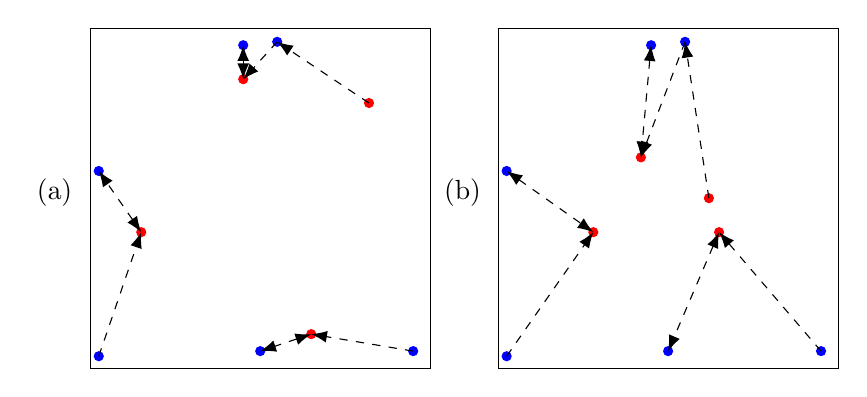
\begin{tikzpicture}[scale=0.00125\textwidth]

    \def\xleft{2};
    \def\xright{14};
    % Draw quarters
    \draw (\xleft,0) rectangle (\xleft+10,10);
    \draw (\xright,0) rectangle (\xright+10,10);

    % Add labels
    \node at (0.95,5.15) {(a)};
    \node at (12.95,5.15) {(b)};

    %set a
    \def\aax{0.25};\def\aay{0.35};
    \def\abx{0.25};\def\aby{5.8};
    \def\acx{5};\def\acy{0.5};
    \def\adx{4.5};\def\ady{9.5};
    \def\aex{5.5};\def\aey{9.6};
    \def\afx{9.5};\def\afy{0.5};
    %set b
    \def\bax{1.5};\def\bay{4};
    \def\bbx{4.5};\def\bby{8.5};
    \def\bcx{6.5};\def\bcy{1};
    \def\bdx{8.2};\def\bdy{7.8};
    %set c
    \def\cax{2.8};\def\cay{4};
    \def\cbx{4.2};\def\cby{6.2};
    \def\ccx{6.2};\def\ccy{5};
    \def\cdx{6.5};\def\cdy{4};



    %set a at a
    \fill[blue] (\xleft+\aax,\aay) circle(.15);
    \fill[blue] (\xleft+\abx,\aby) circle(.15);
    \fill[blue] (\xleft+\acx,\acy) circle(.15);
    \fill[blue] (\xleft+\adx,\ady) circle(.15);
    \fill[blue] (\xleft+\aex,\aey) circle(.15);
    \fill[blue] (\xleft+\afx,\afy) circle(.15);
    %set a at b
    \fill[blue] (\xright+\aax,\aay) circle(.15);
    \fill[blue] (\xright+\abx,\aby) circle(.15);
    \fill[blue] (\xright+\acx,\acy) circle(.15);
    \fill[blue] (\xright+\adx,\ady) circle(.15);
    \fill[blue] (\xright+\aex,\aey) circle(.15);
    \fill[blue] (\xright+\afx,\afy) circle(.15);

     %set b at a
    \fill[red] (\xleft+\bax,\bay) circle(.15);
    \fill[red] (\xleft+\bbx,\bby) circle(.15);
    \fill[red] (\xleft+\bcx,\bcy) circle(.15);
    \fill[red] (\xleft+\bdx,\bdy) circle(.15);

     %set c at b
    \fill[red] (\xright+\cax,\cay) circle(.15);
    \fill[red] (\xright+\cbx,\cby) circle(.15);
    \fill[red] (\xright+\ccx,\ccy) circle(.15);
    \fill[red] (\xright+\cdx,\cdy) circle(.15);


    %drawing line a
    \draw[-{Latex[length=2mm]},dashed] (\xleft+\aax,\aay) -- (\xleft+\bax,\bay);
    \draw[{Latex[length=2mm]}-{Latex[length=2mm]},dashed] (\xleft+\bax,\bay) -- (\xleft+\abx,\aby);
    \draw[{Latex[length=2mm]}-{Latex[length=2mm]},dashed] (\xleft+\bbx,\bby) -- (\xleft+\adx,\ady);
    \draw[{Latex[length=2mm]}-{Latex[length=2mm]},dashed] (\xleft+\bcx,\bcy) -- (\xleft+\acx,\acy);
    \draw[-{Latex[length=2mm]},dashed] (\xleft+\aex,\aey) -- (\xleft+\bbx,\bby);
    \draw[-{Latex[length=2mm]},dashed] (\xleft+\bdx,\bdy) -- (\xleft+\aex,\aey);
    \draw[-{Latex[length=2mm]},dashed] (\xleft+\afx,\afy) -- (\xleft+\bcx,\bcy);

    %drawing line b
    \draw[{Latex[length=2mm]}-{Latex[length=2mm]},dashed] (\xright+\abx,\aby) -- (\xright+\cax,\cay);
    \draw[{Latex[length=2mm]}-{Latex[length=2mm]},dashed] (\xright+\adx,\ady) -- (\xright+\cbx,\cby);
    \draw[{Latex[length=2mm]}-{Latex[length=2mm]},dashed] (\xright+\cdx,\cdy) -- (\xright+\acx,\acy);
    \draw[-{Latex[length=2mm]},dashed] (\xright+\aax,\aay) -- (\xright+\cax,\cay);
    \draw[-{Latex[length=2mm]},dashed] (\xright+\aex,\aey) -- (\xright+\cbx,\cby);
    \draw[-{Latex[length=2mm]},dashed] (\xright+\ccx,\ccy) -- (\xright+\aex,\aey);
    \draw[-{Latex[length=2mm]},dashed] (\xright+\afx,\afy) -- (\xright+\cdx,\cdy);

\end{tikzpicture}
    \caption{Process of obtaining $D_{msw}$}
    \label{fig:msd}
\end{figure}

The similarity equation (equation-\ref{eq:sent_sim}) has a standard deviation $\sigma$ which works
as a control variable and was fine-tuned to be $5 \times 10^{-11}$ where it gave the best results.

\begin{algorithm} \caption{Sentence Similarity Calculation} \label{alg:similarity}
\begin{algorithmic}[1]
    \State $n \gets$ length($VL$)
    \State $A \gets \{ \{0\} \times n \} \times n$
    \For{each sentence$_i$ in $VL$}
        \State $D_{\text{Square}} \gets 0$
        \State count $\gets 0$
        \For{each sentence$_j$ in $VL$}
            \For{each word$_i$ in sentence$_i$}
                \State $D_{\text{msw}} \gets \infty$
                \For{each word$_j$ in sentence$_j$}
                    \If{Distance(word$_i$, word$_j$) $< D_{\text{msw}}$}
                        \State $D_{\text{msw}} \gets$ Distance(word$_i$, word$_j$)
                    \EndIf
                \EndFor
                \State $D_{\text{Square}} \gets D_{\text{Square}} + D_{\text{msw}}^2$
                \State count++
            \EndFor
            \For{each word$_j$ in sentence$_j$}
                \State $D_{\text{msw}} \gets \infty$
                \For{each word$_i$ in sentence$_i$}
                    \If{Distance(word$_i$, word$_j$) $< D_{\text{msw}}$}
                        \State $D_{\text{msw}} \gets$ Distance(word$_i$, word$_j$)
                    \EndIf
                \EndFor
                \State $D_{\text{Square}} \gets D_{\text{Square}} + D_{\text{msw}}^2$
                \State count++
            \EndFor
            \State similarity $\gets \exp \left( \frac{- D_{\text{Square}}}{2 \times \text{count} \times \sigma^2} \right)$
            \State $A[i][j] \gets A[j][i] \gets$ similarity
        \EndFor
    \EndFor
    \State \textbf{Return} $A$
\end{algorithmic}
\end{algorithm}
%\subsubsection{Viability of this strategy}
%To get the similarity between two sentence, we needed a strategy that can match two sets of vectors.
%Other popular methods for the same functionality are also available.
%For example, Earth Mover's Distance (EMD)~\cite{Rubner-19998-emd}, Hausdorff distance, Procrustes Analysis etc.
%EMD tries to find the lowest amount of ``work'' needed to transform one set into the other one.
%This is very computationally expensive.
%And also it focuses on scaling and rotating which are not relevant in word vector space.
%Hausdorff distance takes the worst case scenario and is easily influenced by outliers.
%So, it was avoided.
%Procrustes Analysis tries to find the lowest amount of misalignment after scaling and rotating.
%Both of them are irrelevant in word vector space.\\
%
%On the other hand, our method focuses on Local Point Correspondence between two sets which is more
%important for words.
%The Gaussian similarity function captures the proximity of points smoothly,
%providing continuous feedback on how similar two points are in a normalized way.
%It is also robust against small perturbations because of the use of a soft similarity measure (Gaussian)
%and geometric mean which helps smooth over small differences in point locations.

\subsection{Clustering}\label{subsec:clustering}
The clustering is the most integral part of this summarization technique, aiming to group all the
sentences with similar meanings together.
Here, spectral clustering is used to cluster the sentences using sentence similarity calculated in the step above.
Spectral clustering was chosen here because \citeauthor{roychowdhury-etal-2022-spectral-base}
\cite{roychowdhury-etal-2022-spectral-base} found it to be better performing than DBSCAN method.
The spectral clustering steps were followed according to the tutorial given by
\cite{vonLuxburg-2007-spectral-tutorial}. \\

To perform spectral clustering on a data, firstly, an affinity matrix is required that shows
the weight of edges between the vertexes in the graph.
Here the affinity $A$ is prepared using the following Equation~\ref{eq:affinity}.

\begin{equation}\label{eq:affinity}
    A_{ij}=A_{ji}=Sim(S_i,S_j)
\end{equation}

Here, $S_i, S_j$ are sentences from the input document.
The affinity matrix, $A$, is used in the spectral clustering implementation in the SciKit-learn
tool~\cite{Pedregosa-2011-scikit-learn} in python.
Here, to use the function, we also need to provide the number of clusters to achieve.
The number of clusters are fixed at $k=ceiling\left(\frac{N}{5}\right)$ due to it being a
reasonable size to contain all necessary sentences as well as being short enough to be an effective summary.

\subsection{Summary Generation}\label{subsec:summary-generation}
After clustering, we pick one sentence from each cluster.
The sentences inside a cluster are ranked among themselves using TF-IDF .
The best ranked sentence of the clusters by their order of TF-IDF score is
selected from each cluster.
We then rearranged these picked sentences are in their order of appearance to retain the normal flow of
information in the input.
These sentences are then concatenated together to produce the final output summary.
This is shown in Algorithm~\ref{alg:summary}

\begin{algorithm} \caption{Summary Generation} \label{alg:summary}
\begin{algorithmic}[1]
    \State $k \gets \lceil$ length($A$) / 5 $\rceil$
    \State clusters $\gets$ spectral\_clustering(adjacency = $A$, $k$)
    \State indexes $\gets \{\}$
    \For{each cluster$_i$ in clusters}
        \State TFIDF $\gets \{\}$
        \For{each index in cluster$_i$}
            \State TFIDF.append(tfidf\_sum(sentences[index]))
        \EndFor
        \State indexes.append(indexof(max(TFIDF)))
    \EndFor
    \State sort(indexes)
    \State $S \gets ""$
    \For{each $i$ in indexes}
        \State $S \gets S +$ sentences[$i$]
    \EndFor
    \State \textbf{Return} $S$
\end{algorithmic}
\end{algorithm}



    \section{Result}\label{sec:result}
    The text summarization performance of the proposed model is compared against
the BenSumm~\cite{chowdhury-etal-2021-tfidf-clustering}, LexRank~\cite{Erkan-lexRank-2004} and Sentence
Average Similarity-based Spectral Clustering(SASbSC)-based summarization
method~\cite{roychowdhury-etal-2022-spectral-base} methods.
These methods are the recently published state of the art model for Bengali Extractive Text Summarization.
A classic extractive text summarizing method LexRank~\cite{Erkan-lexRank-2004} was also used as a benchmark for comparison.

\subsection{Evaluation Datasets}\label{subsec:evaluation-datasets}
To examine our proposed model, we compared our model along with the 3 benchmark models on 4 different diverse datasets.
We did this so that the results doesn't become biased due to any problem with the dataset.

\subsubsection{Dataset-1 (Self-curated)}
To evaluate the performance of implemented text summarization
methods~\cite{chowdhury-etal-2021-tfidf-clustering,Erkan-lexRank-2004,roychowdhury-etal-2022-spectral-base},
a curated Bengali extractive text summarization dataset was produced by an expert linguistic team.
250 news documents of various sizes were summarized for this purpose.
Each document was summarized twice by two different person to minimize human bias.
In total, there is 500 different document-summary pair in this dataset.
This dataset is made publicly available\footnote{\textit{dataset link}} for other researchers to use for evaluation
purpose in their research.

\subsubsection{Dataset-2 (Towhid Ahmed Foysal)}
This dataset is a collection of summary article pair from The Daily Prothom Alo.
It was published by Towhid Ahmed Foysal in
Kaggle\footnote{\textit{https://www.kaggle.com/datasets/towhidahmedfoysal/bangla-summarization-datasetprothom-alo}}.
The original dataset was filtered so that all the articles smaller than 50 characters and all the summaries
that contains something not in the original articles were discarded.
After filtering, total 10,204 articles remained, each with 2 summaries.

\subsubsection{Dataset-3 (BNLPC)}
This dataset is a collection of news article summaries published by \citeauthor{Hque-2015-BNLPC-Dataset}~\cite{Hque-2015-BNLPC-Dataset}.
The dataset was collected from
GitHub\footnote{\textit{https://github.com/tafseer-nayeem/BengaliSummarization/tree/main/Dataset/BNLPC/Dataset2}}.
The dataset contains 100 article with 3 different summaries for each article.

\subsubsection{Dataset-4 (Abid Mahdi)}
This dataset was published by Abid Mahdi on
GitHub\footnote{\textit{https://github.com/Abid-Mahadi/Bangla-Text-summarization-Dataset}}.
The dataset contains 200 documents each with 2 summaries.

\subsection{Text Summarization Models}\label{subsec:text-summarization-models}
Four different Bengali extractive text summarization models were implemented to evaluate them by
comparing the machine generated summaries against the human generated summaries from the datasets described above.\\

\textbf{Model-1:} Model-1 is the proposed model for this paper.
The model uses word vector based Gaussian similarity to perform spectral clustering to group similar
sentences together and extract one sentence from each group.
This is described as Word Similarity based Spectral Clustering (WSbSC)\\

\textbf{Model-2:} Model-2 (SASbSC) is the method proposed by \citeauthor{roychowdhury-etal-2022-spectral-base}
\cite{roychowdhury-etal-2022-spectral-base}.
This extractive text summarization method is similar to the proposed method.
SCSbSC method uses the same word embedding dataset as ours to get word vectors.
It uses a sentence center similarity based graph to perform spectral clustering inside the method.
Then use cosine similarity to extract sentences from the input.
To get sentence similarity, SCSbSC averages all the word vectors of a particular sentence to get the Sentence center.
This method was implemented in python as described in their article.\\

\textbf{Model-3:} BenSumm describes two different summarization method in the
study~\cite{chowdhury-etal-2021-tfidf-clustering}.
Here only the extractive method is implemented and compared because the proposed method is also extractive in nature.
BenSumm implements a TF-IDF based cosine similarity graph between the sentences and then clusters the sentences using
Agglomerative Clustering.
The implementation codes are publicly available in
GitHub\footnote{\textit{https://github.com/tafseer-nayeem/BengaliSummarization}}.\\

\textbf{Model-4:} LexRank~\cite{Erkan-lexRank-2004} uses a TF-IDF based Matrix and Googles
PageRank algorithm~\cite{page-PageRank-1999} to rank sentences.
The top ranked sentences are selected and arranged into summary after that.
An implemented version of this method is available as a python package in PyPI as
LexRank\footnote{\textit{https://pypi.org/project/lexrank/}}.
LexRank is applied using a large Bengali Wikipedia
corpus\footnote{\textit{https://www.kaggle.com/datasets/shazol/bangla-wikipedia-corpus}}.

\subsection{Evaluation Metrics}\label{subsec:evaluation-metrics}
To evaluate the correctness of the machine generated summaries compared to the human
generated summaries, we used the ROUGE method~\cite{lin-2004-rouge}.
It compares a human produced reference summary with a machine generated summary.
The ROUGE method uses N-gram based overlapping to find a recall, precision and F-1 score.
The ROUGE implementation that were used is available as a python package in
PyPI\footnote{\textit{https://pypi.org/project/rouge/}}.
There are three different metrics in the package for comparison of the summaries.
These are:

\begin{enumerate}
    \item \textbf{ROUGE-1:} It uses unigram matching to find how much similar two summaries are.
    It is a good first impression for performance but can be misleading too as many large enough texts
    will share very high proportion of uni-grams between them.
    \item \textbf{ROUGE-2:} It uses bi-gram matching to find how much similar the two summaries are in a word level.
    Shared bigrams lead to a deeper analysis of syntactic similarities between the two summaries.
    \item \textbf{ROUGE-LCS:} It finds the longest common sub-sequence between the summaries to calculate
    the rouge scores.
    It can calculate the similarity in flow of the sentences between two summaries.
\end{enumerate}

In this study, we compared the F-1 scores from each of these metrics for the 4 models.

\subsection{Comparison}\label{subsec:comparison}
Average F-1 scores for the three Rouge metrics (Rouge-1, Rouge-2, Rouge-LCS) of the four models(Proposed,
SASbSC, BenSumm, LexRank) on the 4 datasets are shown in the table-\ref{tab:result_comparison-1}. \\

\begin{table}[]
    \centering
    \begin{tabular}{lccc} \hline
         Dataset-1 (SC)                                                 &               &               &               \\
         Model                                                          & Rouge-1       & Rouge-2       & Rouge-LCS     \\\hline
         Model-1 (WSbSC)(Proposed)                                      & \textbf{0.47} & \textbf{0.36} & \textbf{0.43} \\
         Model-2 (BenSumm)~\cite{chowdhury-etal-2021-tfidf-clustering}  & 0.41          & 0.29          & 0.36          \\
         Model-3 (SASbSC)~\cite{roychowdhury-etal-2022-spectral-base}   & 0.42          & 0.29          & 0.37          \\
         Model-4 (LexRank)~\cite{Erkan-lexRank-2004}                          & 0.22          & 0.14          & 0.20          \\\hline
         Dataset-2 (TAF)                                                &               &               &               \\\hline
         Model-1 (WSbSC)(Proposed)                                      & \textbf{0.49} & \textbf{0.43} & \textbf{0.48} \\
         Model-2 (BenSumm)~\cite{chowdhury-etal-2021-tfidf-clustering}  & 0.29          & 0.22          & 0.26          \\
         Model-3 (SASbSC)~\cite{roychowdhury-etal-2022-spectral-base}   & 0.23          & 0.12          & 0.18          \\
         Model-4 (LexRank)~\cite{Erkan-lexRank-2004}                          & 0.24          & 0.16          & 0.22          \\\hline
         Dataset-3 (BNLPC)                                              &               &               &               \\\hline
         Model-1 (WSbSC)(Proposed)                                      & \textbf{0.41} & \textbf{0.34} & \textbf{0.40} \\
         Model-2 (BenSumm)~\cite{chowdhury-etal-2021-tfidf-clustering}  & 0.36          & 0.28          & 0.34          \\
         Model-3 (SASbSC)~\cite{roychowdhury-etal-2022-spectral-base}   & \textbf{0.41} & 0.33          & 0.39          \\
         Model-4 (LexRank)~\cite{Erkan-lexRank-2004}                          & 0.26          & 0.19          & 0.24          \\\hline
         Dataset-4 (AM)                                                 &               &               &               \\\hline
         Model-1 (WSbSC)(Proposed)                                      & \textbf{0.49} & \textbf{0.41} & \textbf{0.47} \\
         Model-2 (BenSumm)~\cite{chowdhury-etal-2021-tfidf-clustering}  & 0.31          & 0.22          & 0.28          \\
         Model-3 (SASbSC)~\cite{roychowdhury-etal-2022-spectral-base}   & 0.30          & 0.18          & 0.24          \\
         Model-4 (LexRank)~\cite{Erkan-lexRank-2004}                          & 0.22          & 0.14          & 0.20          \\
    \end{tabular}
    \caption{Comparison of average Rouge scores between graph based extractive summarization models on 4 different datasets}
    \label{tab:result_comparison-1}
\end{table}

These results are further summarized into 3 radar charts so that the performance of each model on each
metric for the datasets can be visualized.

\begin{figure}
    \centering
    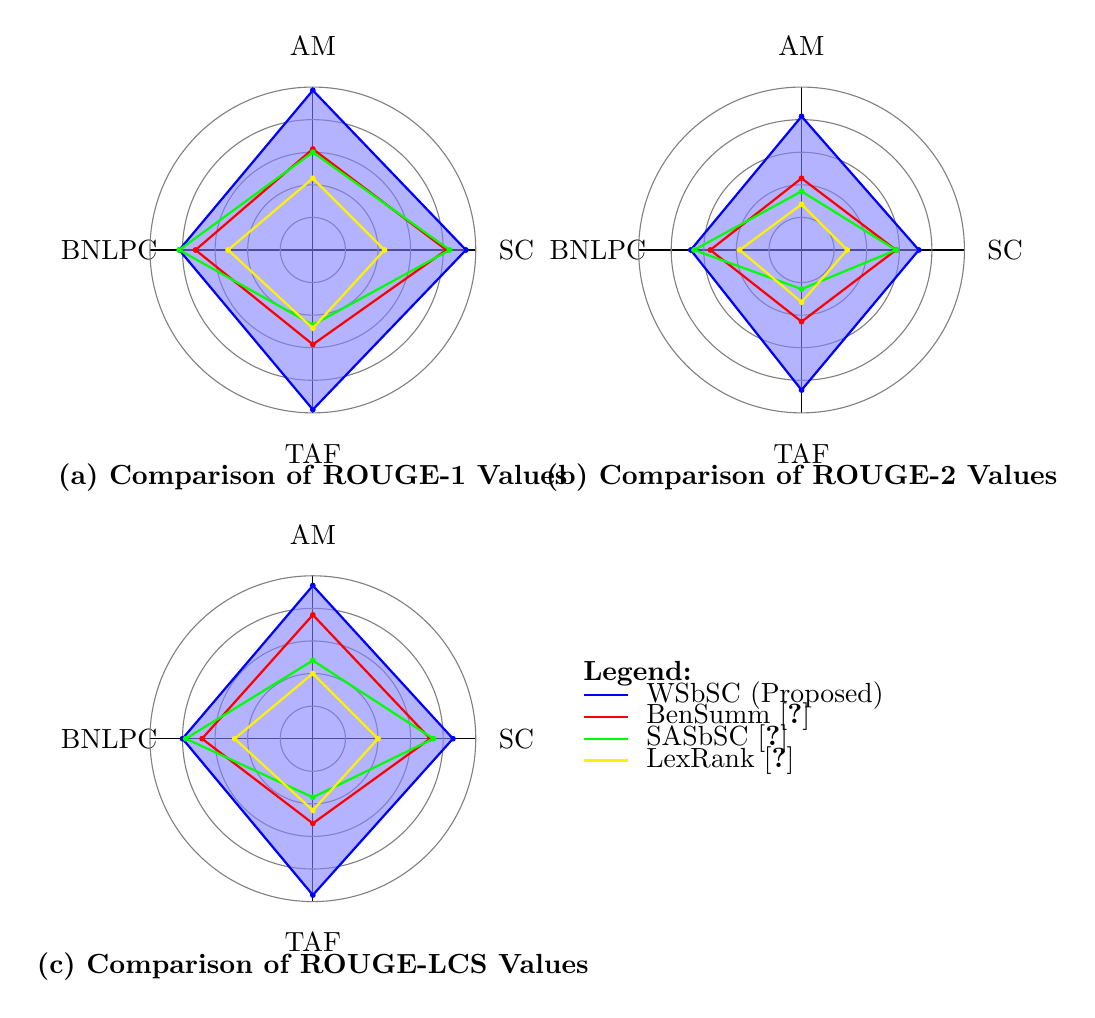
\begin{tikzpicture}[scale=0.002*\textwidth]
    % Define the number of axes (dimensions)
    \def\n{4}
    % Define the names of the features
    \def\features{{"SC", "TAF", "BNLPC", "AM"}}
    % Define the maximum value
    \def\maxvalue{5}

    % Define values for three different radar charts
    \def\valuesAW{{4.7, 4.9, 4.1, 4.9}}
    \def\valuesAB{{4.1, 2.9, 3.6, 3.1}}
    \def\valuesAS{{4.2, 2.3, 4.1, 3.0}}
    \def\valuesAL{{2.2, 2.4, 2.6, 2.2}}

    \def\valuesBW{{3.6, 4.3, 3.4, 4.1}}
    \def\valuesBB{{2.9, 2.2, 2.8, 2.2}}
    \def\valuesBS{{2.9, 1.2, 3.3, 1.8}}
    \def\valuesBL{{1.4, 1.6, 1.9, 1.4}}

    \def\valuesCW{{4.3, 4.8, 4.0, 4.7}}
    \def\valuesCB{{3.6, 2.6, 3.4, 3.8}}
    \def\valuesCS{{3.7, 1.8, 3.9, 2.4}}
    \def\valuesCL{{2.0, 2.2, 2.4, 2.0}}

    % First Radar Chart (Top-left quarter)
    \begin{scope}[xshift=-5cm, yshift=5cm, scale=0.6]
        %write the dataset labels
        \foreach \i in {1,...,\n} {
            \draw (90-\i*360/\n:5) -- (0,0);
            \node at (90-\i*360/\n:6.25) {\pgfmathparse{\features[\i-1]}\pgfmathresult};
        }
        %draw the circle
        \node at (90-2*360/4:7){\textbf{(a) Comparison of ROUGE-1 Values}};
        \foreach \j in {1,...,\maxvalue} {
            \draw[gray, thin] (0,0) circle (\j);
        }

        %draw wsbsc
        \foreach \i [evaluate={\angle=90-\i*360/\n; \valueAW=\valuesAW[\i-1];}] in {1,...,\n} {
            \coordinate (PA\i) at (\angle:\valueAW);
            \filldraw[blue] (PA\i) circle (2pt);
        }
        \fill[blue!50, opacity=0.6] (PA1) -- (PA2) -- (PA3) -- (PA4) -- cycle;
        \foreach \i in {1,...,\n} {
            \pgfmathtruncatemacro{\nexti}{mod(\i,\n)+1}
%                    \draw [thick, cyan] plot [smooth, tension=2] coordinates { (PA\i) (PA\nexti)};
            \draw[thick, blue] (PA\i) -- (PA\nexti);
        }
%                \draw [thick,cyan] plot [smooth cycle, tension=1] coordinates { (PA1) (PA2) (PA3) (PA4)};

        %draw bensumm
        \foreach \i [evaluate={\angle=90-\i*360/\n; \valueAB=\valuesAB[\i-1];}] in {1,...,\n} {
            \coordinate (PB\i) at (\angle:\valueAB);
            \filldraw[red] (PB\i) circle (2pt);
        }
        \foreach \i in {1,...,\n} {
            \pgfmathtruncatemacro{\nexti}{mod(\i,\n)+1}
            \draw[thick, red] (PB\i) -- (PB\nexti);
        }

%                draw sasbsc
        \foreach \i [evaluate={\angle=90-\i*360/\n; \valueAS=\valuesAS[\i-1];}] in {1,...,\n} {
            \coordinate (PC\i) at (\angle:\valueAS);
            \filldraw[green] (PC\i) circle (2pt);
        }
        \foreach \i in {1,...,\n} {
            \pgfmathtruncatemacro{\nexti}{mod(\i,\n)+1}
            \draw[thick, green] (PC\i) -- (PC\nexti);
        }

        %draw lexrank
        \foreach \i [evaluate={\angle=90-\i*360/\n; \valueAL=\valuesAL[\i-1];}] in {1,...,\n} {
            \coordinate (PD\i) at (\angle:\valueAL);
            \filldraw[yellow] (PD\i) circle (2pt);
        }
        \foreach \i in {1,...,\n} {
            \pgfmathtruncatemacro{\nexti}{mod(\i,\n)+1}
            \draw[thick, yellow] (PD\i) -- (PD\nexti);
        }
    \end{scope}

    % Second Radar Chart (Top-right quarter)
    \begin{scope}[xshift=4cm, yshift=5cm, scale=0.6]
        \foreach \i in {1,...,\n} {
            \draw (90-\i*360/\n:5) -- (0,0);
            \node at (90-\i*360/\n:6.25) {\pgfmathparse{\features[\i-1]}\pgfmathresult};
        }
        \node at (90-2*360/4:7){\textbf{(b) Comparison of ROUGE-2 Values}};
        \foreach \j in {1,...,\maxvalue} {
            \draw[gray, thin] (0,0) circle (\j);
        }

        \foreach \i [evaluate={\angle=90-\i*360/\n; \valueBW=\valuesBW[\i-1];}] in {1,...,\n} {
            \coordinate (PA\i) at (\angle:\valueBW);
            \filldraw[blue] (PA\i) circle (2pt);
        }
        \fill[blue!50, opacity=0.6] (PA1) -- (PA2) -- (PA3) -- (PA4) -- cycle;
        \foreach \i in {1,...,\n} {
            \pgfmathtruncatemacro{\nexti}{mod(\i,\n)+1}
            \draw[thick, blue] (PA\i) -- (PA\nexti);
        }

        \foreach \i [evaluate={\angle=90-\i*360/\n; \valueBB=\valuesBB[\i-1];}] in {1,...,\n} {
            \coordinate (PB\i) at (\angle:\valueBB);
            \filldraw[red] (PB\i) circle (2pt);
        }
        \foreach \i in {1,...,\n} {
            \pgfmathtruncatemacro{\nexti}{mod(\i,\n)+1}
            \draw[thick, red] (PB\i) -- (PB\nexti);
        }

        \foreach \i [evaluate={\angle=90-\i*360/\n; \valueBS=\valuesBS[\i-1];}] in {1,...,\n} {
            \coordinate (PC\i) at (\angle:\valueBS);
            \filldraw[green] (PC\i) circle (2pt);
        }
        \foreach \i in {1,...,\n} {
            \pgfmathtruncatemacro{\nexti}{mod(\i,\n)+1}
            \draw[thick, green] (PC\i) -- (PC\nexti);
        }

        \foreach \i [evaluate={\angle=90-\i*360/\n; \valueBL=\valuesBL[\i-1];}] in {1,...,\n} {
            \coordinate (PD\i) at (\angle:\valueBL);
            \filldraw[yellow] (PD\i) circle (2pt);
        }
        \foreach \i in {1,...,\n} {
            \pgfmathtruncatemacro{\nexti}{mod(\i,\n)+1}
            \draw[thick, yellow] (PD\i) -- (PD\nexti);
        }
    \end{scope}

    % Third Radar Chart (Bottom-left quarter)
    \begin{scope}[xshift=-5cm, yshift=-4cm, scale=0.6]
        \foreach \i in {1,...,\n} {
            \draw (90-\i*360/\n:5) -- (0,0);
            \node at (90-\i*360/\n:6.25) {\pgfmathparse{\features[\i-1]}\pgfmathresult};
        }
        \node at (90-2*360/4:7){\textbf{(c) Comparison of ROUGE-LCS Values}};
        \foreach \j in {1,...,\maxvalue} {
            \draw[gray, thin] (0,0) circle (\j);
        }

        \foreach \i [evaluate={\angle=90-\i*360/\n; \valueCW=\valuesCW[\i-1];}] in {1,...,\n} {
            \coordinate (PA\i) at (\angle:\valueCW);
            \filldraw[blue] (PA\i) circle (2pt);
        }
        \fill[blue!50, opacity=0.6] (PA1) -- (PA2) -- (PA3) -- (PA4) -- cycle;
        \foreach \i in {1,...,\n} {
            \pgfmathtruncatemacro{\nexti}{mod(\i,\n)+1}
            \draw[thick, blue] (PA\i) -- (PA\nexti);
        }

        \foreach \i [evaluate={\angle=90-\i*360/\n; \valueCB=\valuesCB[\i-1];}] in {1,...,\n} {
            \coordinate (PB\i) at (\angle:\valueCB);
            \filldraw[red] (PB\i) circle (2pt);
        }
        \foreach \i in {1,...,\n} {
            \pgfmathtruncatemacro{\nexti}{mod(\i,\n)+1}
            \draw[thick, red] (PB\i) -- (PB\nexti);
        }

        \foreach \i [evaluate={\angle=90-\i*360/\n; \valueCS=\valuesCS[\i-1];}] in {1,...,\n} {
            \coordinate (PC\i) at (\angle:\valueCS);
            \filldraw[green] (PC\i) circle (2pt);
        }
        \foreach \i in {1,...,\n} {
            \pgfmathtruncatemacro{\nexti}{mod(\i,\n)+1}
            \draw[thick, green] (PC\i) -- (PC\nexti);
        }

        \foreach \i [evaluate={\angle=90-\i*360/\n; \valueCL=\valuesCL[\i-1];}] in {1,...,\n} {
            \coordinate (PD\i) at (\angle:\valueCL);
            \filldraw[yellow] (PD\i) circle (2pt);
        }
        \foreach \i in {1,...,\n} {
            \pgfmathtruncatemacro{\nexti}{mod(\i,\n)+1}
            \draw[thick, yellow] (PD\i) -- (PD\nexti);
        }
    \end{scope}

    % Legend (Bottom-right quarter)
    \begin{scope}[xshift=4cm, yshift=-4cm, scale=0.8]
        \node[anchor=west] at (-5.25, 1.5) {\textbf{Legend:}};
        \draw[thick, blue] (-5, 1) -- (-4, 1);
        \node[anchor=west] at (-3.8, 1) {WSbSC (Proposed)};

        \draw[thick, red] (-5, 0.5) -- (-4, 0.5);
        \node[anchor=west] at (-3.8, 0.5) {BenSumm~\cite{chowdhury-etal-2021-tfidf-clustering}};

        \draw[thick, green] (-5, 0) -- (-4, 0);
        \node[anchor=west] at (-3.8, 0) {SASbSC~\cite{roychowdhury-etal-2022-spectral-base}};

        \draw[thick, yellow] (-5, -0.5) -- (-4, -0.5);
        \node[anchor=west] at (-3.8, -0.5) {LexRank~\cite{Erkan-lexRank-2004}};
    \end{scope}
\end{tikzpicture}
    \caption{Radar chart of the models being compared on 3 different metrics and 4 datasets.}
    \label{fig:radarchart}
 \end{figure}

These charts (Figure~\ref{fig:radarchart}) shows us that the proposed method is much more dataset independent and performs
uniformly on every metric across the datasets.
Other models although performs good on certain datasets, fails to show consistency.

\subsection{Different Ranking Techniques Inside Clusters}\label{subsec:different-ranking-techniques-inside-clusters}
We implemented two ranking methods to pick the best sentence from each clusters.
First one is the First Rank method where we just pick the sentence that is first in terms of their order of
appearance inside the input document.
The second one is the TF-IDF ranking, where we ranked the sentences by their TF-IDF scores and pick the best one.
We can see in the table~\ref{tab:ranking} that the TF-IDF scores better on a high quality dataset like our Self-curated one.

\begin{table}\label{tab:ranking}
    \centering
    \begin{tabular}{cccc}\hline
        Method      & Rouge-1       & Rouge-2       & Rouge-LCS     \\\hline
        FirstRank   & 0.47          & 0.36          & 0.43          \\
        TF-IDF      & \textbf{0.50} & \textbf{0.40} & \textbf{0.46} \\\hline
    \end{tabular}
    \caption{Comparison of Result of different ranking techniques}
\end{table}

\subsection{Implementation Into Other Languages}\label{subsec:implementation-into-other-languages}
The model discussed here is not language dependent.
So the model can be easily extended into other languages.
To perform this method into a language, we only need a language specific tokenizer, a list of stop-words and
a word vector embedding dataset.
We tried to find quality extractive text summarization dataset for evaluating the method, but could only
find relevant datasets on 3 other languages.
These are Hindi, Marathi and Turkish.
We adopted this Model into these 3 low resource languages to check this hypothesis.\\

\begin{table}
    \centering
    \begin{tabular}{cccc}\hline
        Language                & Rouge-1   & Rouge-2   & Rouge-LCS \\\hline
        Bengali (Dataset - 1)   & 0.47      & 0.36      & 0.43      \\
        Bengali (Dataset - 2)   & 0.49      & 0.43      & 0.48      \\
        Bengali (Dataset - 3)   & 0.41      & 0.34      & 0.40      \\
        Bengali (Dataset - 4)   & 0.49      & 0.41      & 0.47      \\
        Bengali (Average)       & 0.47      & 0.38      & 0.44      \\\hline
        Hindi                   & 0.40      & 0.26      & 0.36      \\\hline
        Marathi                 & 0.50	    & 0.42      & 0.50      \\\hline
        Turkish                 & 0.48      & 0.39      & 0.47      \\\hline
    \end{tabular}
    \caption{Comparison of Result of proposed summarization method in other low-resource languages}
    \label{tab:other_language}
\end{table}

The Table-\ref{tab:other_language} shows the result of the proposed word similarity based spectral clustering
method for extractive summarization in other low resource languages.
For the Hindi language, we used a Kaggle
dataset\footnote{\textit{https://www.kaggle.com/datasets/disisbig/hindi-text-short-and-large-summarization-corpus/}}
produced by Gaurav Arora.
For the Marathi language we used another Kaggle
dataset\footnote{\textit{https://www.kaggle.com/datasets/ketki19/marathi}} produced by Ketki Nirantar.
For the Turkish language we used a Github
dataset\footnote{\textit{https://github.com/xtinge/turkish-extractive-summarization-dataset/blob/main/dataset/XTINGE-SUM\_TR\_EXT/xtinge-sum\_tr\_ext.json}}
produced by the XTINGE~\cite{Demir-2024-xtinge_turkish_extractive} team.
We can see that the results remain very close despite the change in language.




    \section{Discussion}\label{sec:discussion}
    The results presented in the previous sections highlight the effectiveness of the
proposed Word Similarity-based Spectral Clustering (WSbSC) model for extractive text summarization
in Bengali, as well as its adaptability to other low-resource languages.
This section delves into an analysis of the comparative results, the strengths and limitations of the proposed method,
and potential areas for further research.\\

As evidenced by the results shown in Table~\ref{tab:result_comparison-1} and Figure~\ref{fig:radarchart},
the WSbSC model consistently outperforms the baseline models,
namely BenSumm~\cite{das-2022-tfidf}, LexRank~\cite{Erkan-lexRank-2004}, and Sentence Average Similarity-based
Spectral Clustering (SASbSC)~\cite{roychowdhury-etal-2022-spectral-base}, across multiple datasets.
This performance improvement is largely for the novel approach of calculating sentence similarity.
Taking the geometric means of individual word similarities overcomes the problems of averaging vector method.
The Gaussian similarity-based approach used in WSbSC provides a more novel and precise method for
capturing the semantic relationships between sentences.\\
%The superior performance of WSbSC is especially noticeable in terms of ROUGE scores,
%where it consistently achieves higher F-1 scores across all datasets (Table~\ref{tab:result_comparison-1}).
%This suggests that the proposed method generates summaries that are more faithful to the
%human written reference summaries.
%Additionally, the clustering approach makes sure that sentences with similar information
%are grouped together, allowing the model to pick the most representative sentence from each group.
%This reduces redundancy and increases topic coverage, key components of a good summary.\\

Our proposed strategy is more suited for the sentence similarity calculation
than other strategies that can compare two sets of vectors
such as Earth Movers Distance (EMD)~\cite{Rubner-19998-emd},
Hausdorff Distance~\cite{hausdorff-1914-hausdorff-distance},
Procrustes Analysis~\cite{Gower-1975-procrustes-distance}.
EMD~\cite{Rubner-19998-emd} tries to find the lowest amount of ``work'' needed to transform one set into the other one.
It considers adding a new point to a set, removing a point from a set,
scaling the whole set, moving a point, rotating the set etc.\ as ``work''.
This is very computationally expensive as hundreds of separate possibilities have to be checked for each
point in each set.
And it also focuses on scaling and rotating, which are not relevant in word vector space.
Another method, Hausdorff distance~\cite{hausdorff-1914-hausdorff-distance} takes the worst case scenario
and calculates the farthest distance between two points in the two set.
It is easily influenced by outliers.
It was avoided because words tend to spread out over the whole word space and this would suffer
from the same problem as the averaging method.
Procrustes Analysis~\cite{Gower-1975-procrustes-distance} tries to find the lowest
amount of misalignment after scaling and rotating the two sets.
Both of these processes are irrelevant in the context of word vector.\\

On the other hand, the proposed method focuses on Local Point Correspondence between
two sets which is more important for words.
The Gaussian similarity function captures the proximity of points smoothly,
providing continuous feedback on how similar two points are in a normalized way.
It is also robust against small outliers because of the use of a soft similarity measure (Gaussian)
and geometric mean which helps smooth over small differences in word similarities.\\

One of the key strengths of this proposed method is the reduction of redundancy,
which is a common issue in extractive summarization methods.
By grouping sentences with similar meanings and selecting a representative
sentence from each group, the model ensures that the summary covers
a broad range of topics without repeating itself.
The use of Spectral clustering is well-suited for the clustering task too
because it does not assume a specific cluster shape
and can infer the number of clusters using the Eigen gap method.
Our proposed model also has an improved sentence similarity calculation technique.
Using the geometric mean of individual word similarities offers a more precise measure
of how closely two sentences are related.
This is a marked improvement over traditional methods that
rely on word averaging, which often dilute the semantic meaning of a sentence.
Another key strength is that it is found to be scalable across languages.
By requiring only a language-specific tokenizer, stop-word list, and word embedding dataset,
WSbSC can be easily adapted to other languages, as demonstrated in the experiments with
Hindi, Marathi, and Turkish datasets (Table~\ref{tab:other_language}).
This makes the model highly versatile and valuable for extractive summarization in low-resource languages.\\

Despite its advantages, the WSbSC model does face some challenges.
The model heavily relies on pre-trained word embeddings,
which may not always capture the full details of certain domains or newly coined terms.
The FastText~\cite{grave-etal-2018-fasttext} dataset used here is
heavily reliant on wikipedia for training.
Which could introduce some small unforeseen biases.
In cases where the word embeddings do not fully have some word of a given document,
the model’s performance could degrade as it leaves those words out.
The model also does not take into account the order in which words appear in a sentence
or when the form special noun or verb groups.
So it can be a little naive in some highly specialized fields.\\

The WSbSC model has demonstrated its ability to perform well in low-resource languages
such as Hindi, Marathi, and Turkish.
Despite differences in language structure, the model’s core methodology remained effective,
yielding results that were consistent with the Bengali dataset evaluations.
This underscores the potential of WSbSC as a generalizable approach
for extractive summarization across different languages, if
appropriate pre-processing tools and word embedding datasets are available.\\

The proposed Word Similarity-based Spectral Clustering model represents a
significant advancement in Bengali extractive text summarization.
Its ability to accurately capture sentence similarity, reduce redundancy, and generalize
across languages makes it a valuable tool for summarizing text in low-resource languages.
While there are still challenges to be addressed, the results of this study demonstrate the
robustness and adaptability of the WSbSC model, offering a promising direction for future research
in multilingual extractive summarization.


    \section{Conclusion}\label{sec:conclusion}
    
In this study, we proposed and evaluated a Word Similarity-based Spectral Clustering (WSbSC)
method for Bengali extractive text summarization.
The method uses semantic relationships between words to
identify the best sentences from a text, addressing the need for
effective summarization techniques in the Bengali language,
which remains underrepresented in natural language processing research.
By using spectral clustering,
we aimed to group sentences based on their semantic similarity,
improving the coherence and relevance of the generated summaries.\\

Through extensive experimentation on different Bengali summarization datasets,
our results showed that the WSbSC method outperforms several baseline techniques,
particularly in grouping the sentences into key topics of documents.
Despite these promising results,
there are areas of further improvement.
One limitation observed is that the method may struggle with highly
specialized or domain-specific texts,
where deeper linguistic features beyond word similarity could be considered.
Future work could explore hybrid models that integrate other
post-processing techniques to improve the output.\\

In conclusion, this work contributes to the growing body of computational
linguistics research focused on low-resource languages like Bengali.
The WSbSC method offers a novel approach for extractive summarization
and sets the stage for further advancements in both Bengali text processing
and multilingual summarization techniques.





    \bibliography{bib/main}
    \bibliographystyle{plainnat}



\end{document}
